\documentclass[aspectratio=169]{beamer}
\PassOptionsToPackage{english}{babel}
\usepackage{standardslides}

\usepackage{tikz}
\usepackage{pifont}
\usepackage{listings}
\usepackage{colortbl}
\newlength{\listingframemargin}
\setlength{\listingframemargin}{1em}
\newlength{\listingmargin}
\setlength{\listingmargin}{0.08\textwidth}

\definecolor{codeDarkGray}{gray}{0.2}
\definecolor{codeGray}{gray}{0.4}
\definecolor{codeLightGray}{rgb}{0.94,0.94,0.91}
\definecolor{codeBorder}{rgb}{0.34,0.24,0.21}
\definecolor{MidnightBlue}{rgb}{0.1, 0.1, 0.8}

\lstdefinestyle{standard}{%
  belowcaptionskip=0.5\baselineskip,
  breaklines=true,
  frameround=tttt,
  % frame=false,
  xleftmargin=0em,
  xrightmargin=0em,
  showstringspaces=false,
  showtabs=false,
  % tab=\smash{\rule[-.2\baselineskip]{.4pt}{\baselineskip}\kern.5em},
  basicstyle= \fontfamily{pcr}\selectfont\scriptsize\bfseries,
  keywordstyle= \bfseries\color{MidnightBlue}, %\color{codeDarkGray},
  commentstyle= \itshape\color{codeGray},
  identifierstyle=\color{codeDarkGray},
  stringstyle=\color{BurntOrange}, %\color{codeDarkGray},
  numberstyle=\tiny\ttfamily,
  % numbers=left,
  numbersep = 1em,
  % stepnumber = 1,
  % captionpos=t,
  tabsize=2,
  % backgroundcolor=\color{codebLightGray},
  rulecolor=\color{codeBorder},
  framexleftmargin=\listingframemargin,
  framexrightmargin=\listingframemargin
}

\newcommand{\inputCodeBlock}[1]{%
  % \begin{mybox}
    \begin{center}
      % \begin{minipage}[c]{0.7\textwidth}
        \lstinputlisting[%
          style = standard,
          language = c++,
          morekeywords={constexpr,noexcept,decltype,size_t,uint32_t,uint64_t,__m256i,__m256,__m256d,__m128i,__m128,__m128d}
        ]{#1}
      % \end{minipage}
    \end{center}
  % \end{mybox}
}

\def\UrlBigBreaks{\do\/\do-\do:}

\title{%
  Algorithmical Geometry: Delaunay Triangulation%
}
% \subtitle{Master's Thesis Defense and Presentation}
\author{Markus Pawellek}

\bibliography{references}

\begin{document}

\selectlanguage{english}

{ % all template changes are local to this group.
  \setbeamertemplate{navigation symbols}{}
  \begin{frame}<article:0>[plain]
    \begin{tikzpicture}[remember picture,overlay]
      \node[at=(current page.center)] {
        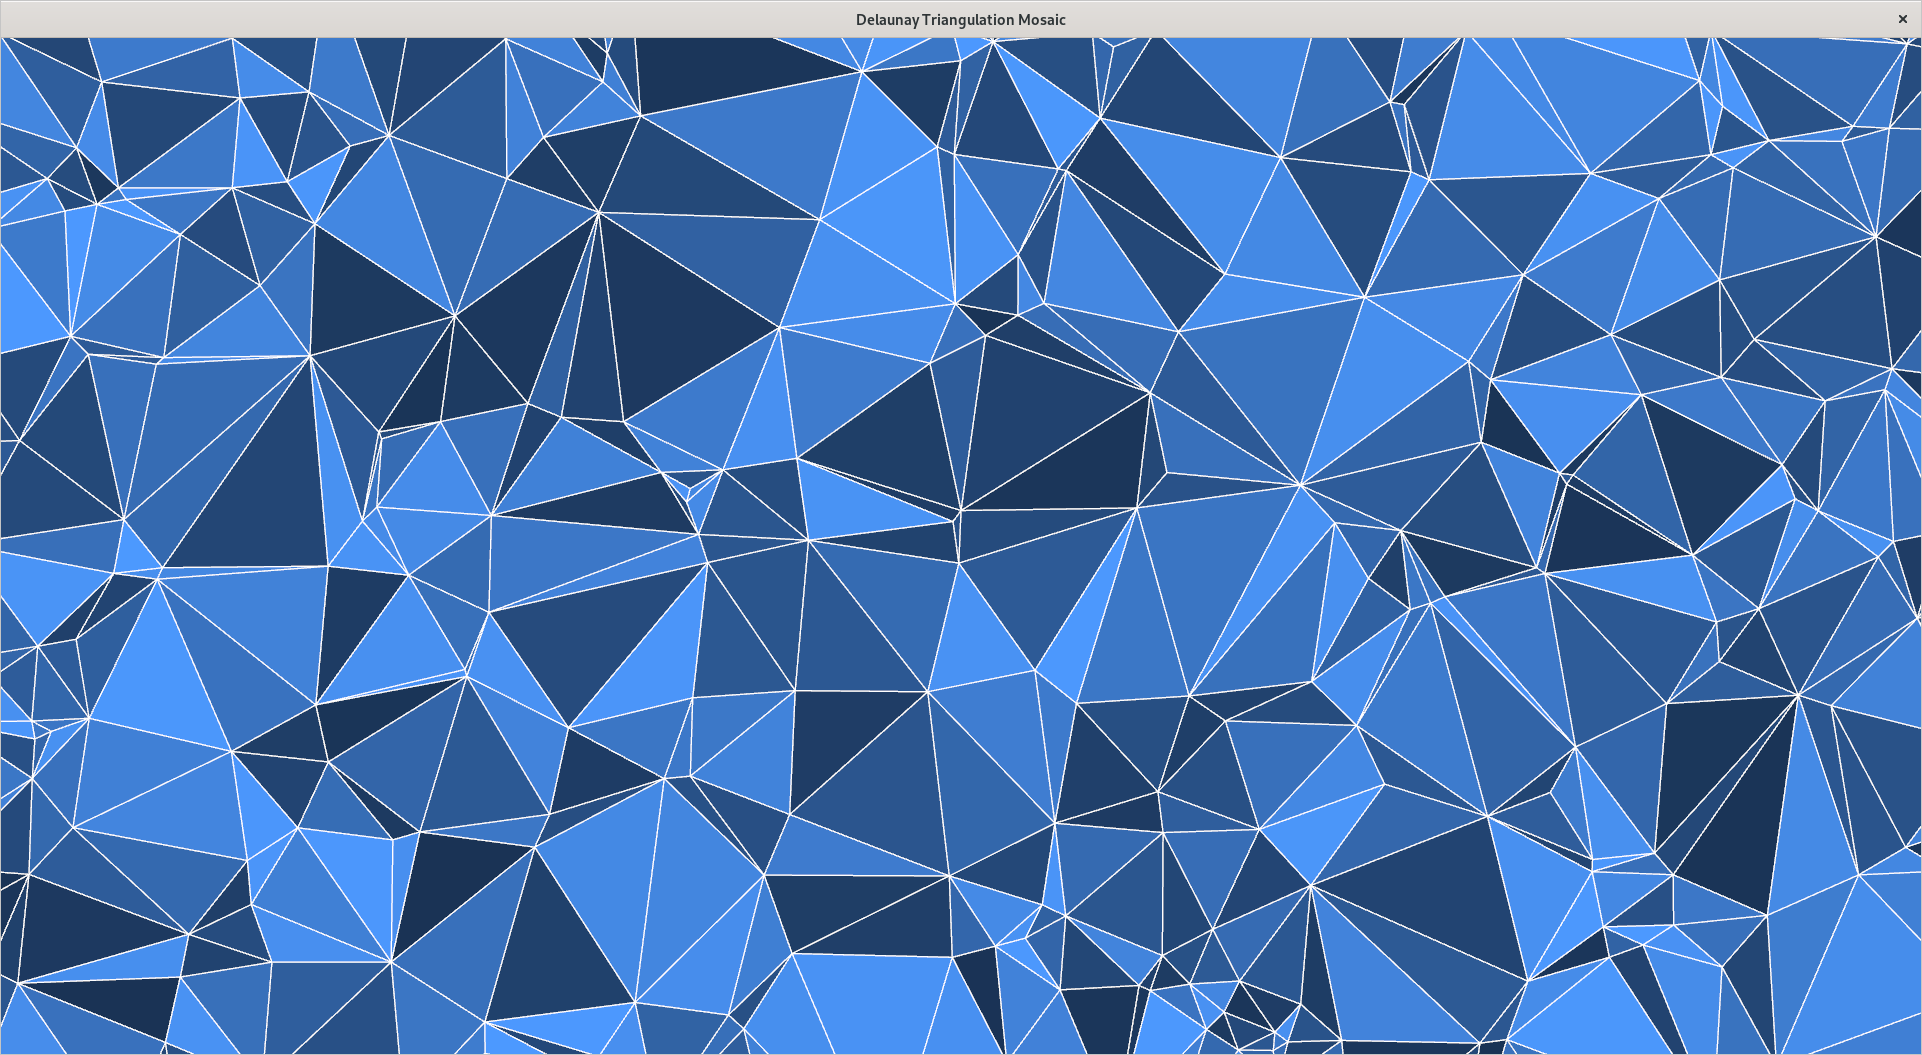
\includegraphics[keepaspectratio,
                         width=1.2\paperwidth,
                         height=\paperheight]{images/banner.png}
      };
    \end{tikzpicture}
  \end{frame}
}

\frame{\titlepage}
\begin{frame}{Outline}
  \footnotesize
  \hfill\parbox[t][7cm][l]{0.9\textwidth}{\tableofcontents}
\end{frame}

\section{Introduction}
\begin{frame}{Introduction: Previous Work and Hands-On Approach}
  \begin{description}
    % This custom command does not work...
    % \newcommand\mycommand[1]{\item[\autocite{#1}] \citeauthor{#1}, \citetitle{#1}, \citeyear{#1}}
    \item[\autocite{shewchuk1996}] \citeauthor{shewchuk1996}, \citetitle{shewchuk1996}, \citeyear{shewchuk1996}
    \item[\autocite{guibas1985}] \citeauthor{guibas1985}, \citetitle{guibas1985}, \citeyear{guibas1985}
    \item[\autocite{dwyer1987}] \citeauthor{dwyer1987}, \citetitle{dwyer1987}, \citeyear{dwyer1987}
    \item[\autocite{lee1980}] \citeauthor{lee1980}, \citetitle{lee1980}, \citeyear{lee1980}
  \end{description}
\end{frame}

\begin{frame}{Introduction: Overview}
  Educational Problems:
  \begin{itemize}
    \item Duality to Voronoi Diagrams, Dirichlet
    \item Incremental, Sweepline, Divide-and-Conquer Algorithms
    \item Varying Data Structures
  \end{itemize}
  \bigskip
  Here: Triangular Data Structure and Divide-and-Conquer Algorithm
  \begin{itemize}
    \item Smallest Data Structure
    \item Fastest Algorithm
    \item Robust when using tweaks
  \end{itemize}
\end{frame}

\section{Background}
\begin{frame}{Background: Triangle}
  % Definition of a triangle can be difficult.
  % Hence, we use and indirect approach.
  \begin{minipage}[c]{0.45\textwidth}
    Definition: (Triangle)\\
    We say that three points $A, B, C \in \setReal^2$ are building a triangle if they are affine independent.
    \bigskip

    Definition: (Circumcircle)\\
    If $A, B, C \in \setReal^2$ are building a triangle, we define the circumcircle of the built triangle to be the circle that intersects with $A$, $B$, and $C$.
    We call its center the circumcenter of the triangle.
  \end{minipage}
  \hfill
  \begin{minipage}[c]{0.49\textwidth}
    \centering
    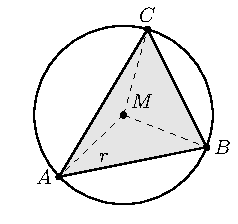
\includegraphics[width=0.9\textwidth]{figures/triangle-circumcirle.pdf}
  \end{minipage}
\end{frame}

\begin{frame}{Background: Triangulation}
  Definition: (Triangulation)
  \begin{itemize}
    \item $n\in\setNatural, n\geq 3$
    \item $\forall i\in\setNatural, i \leq n: \quad x_i \in \setReal^2$ affine independent
    \item $\mathscr{V}\define \set{x_i}{i\in\setNatural, i \leq n}$
    \item $\mathscr{T}(\mathscr{V})$ is a planar graph such that all faces are triangles when vertices are drawn at their given positions.
    \item $\mathscr{DT}(\mathscr{V})$ is a Delaunay triangulation if it is a triangulation such that for all triangle faces the interior of the circumcircle contains no other points of $\mathscr{V}$.
  \end{itemize}
\end{frame}

\begin{frame}{Background: Properties of Delaunay Triangulation}
  \begin{itemize}
    \item Duality to Voronoi Diagram
    \item always exists
    \item If no points are cocircular, unique
    \item optimality: maximization of the minimum angle of all angles
    \item boundary is convex hull
    \item Delaunay condition implies triangulation
  \end{itemize}
\end{frame}

\begin{frame}{Background: Existence and Uniqueness of Delaunay Triangulation}
  % algorithms may already be a proof
  % maybe by induction
  % edge-flip
\end{frame}

\section{Geometric Primitives}
\begin{frame}{Geometric Primitives: Counter-Clockwise}
  \[
    \begin{vmatrix}
      A_x & A_y & 1 \\
      B_x & B_y & 1 \\
      C_x & C_y & 1 \\
    \end{vmatrix}
    > 0
  \]
\end{frame}

\begin{frame}{Geometric Primitives: Inside Circumcircle}
  \[
    \begin{vmatrix}
      A_x & A_y & A_x^2 + A_y^2 & 1 \\
      B_x & B_y & B_x^2 + B_y^2 & 1 \\
      C_x & C_y & C_x^2 + C_y^2 & 1 \\
      D_x & D_y & D_x^2 + D_y^2 & 1 \\
    \end{vmatrix}
    > 0
  \]
\end{frame}

\section{Data Structures}

\section{Algorithm}

\section{Implementation}
\begin{frame}{Implementation}
  \begin{itemize}
    \item Geometric Primitives need exact computation and therefore arbitrary precision
  \end{itemize}
\end{frame}

\section{Applications}

\section{Conclusions}

\begin{frame}
  \vfill
  \centering
  \begin{beamercolorbox}[sep=8pt,center,shadow=true,rounded=true]{title}
    \usebeamerfont{title}%
    Thank you for Your Attention!%
    \par%
  \end{beamercolorbox}
  \vfill
\end{frame}

\begin{frame}
  \frametitle{References}
  % \tiny
  \AtNextBibliography{\tiny}
  \begin{multicols}{2}
    \nocite{*}
    \printbibliography
  \end{multicols}
\end{frame}

\end{document}
